\subsection*{1−1インターネットのキホン}
\refstepcounter{PagePtr}\label{P:internet}
\begin{wrapfigure}{r}[10pt]{0.4\textwidth}
	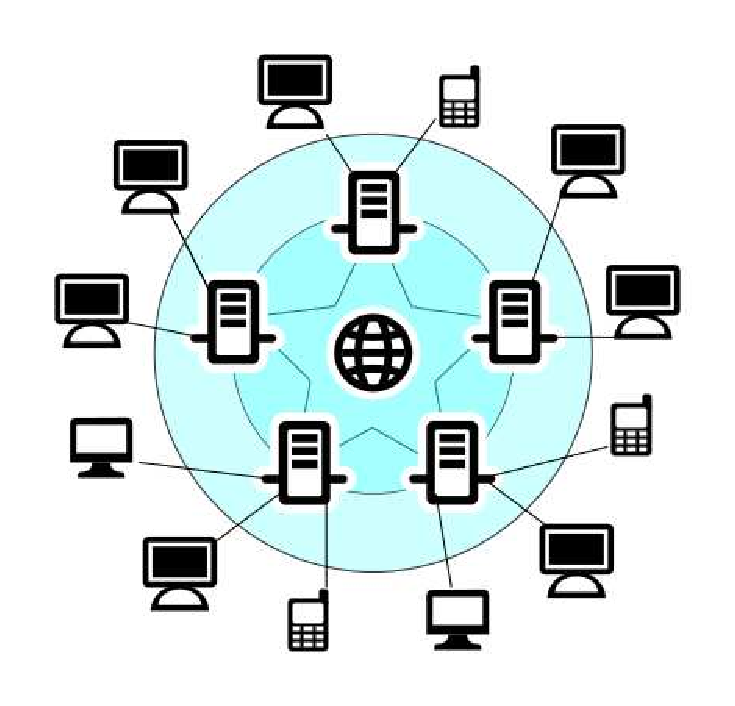
\includegraphics[width=0.4\textwidth]{text07-img/ome7-img002.eps}
\end{wrapfigure}

みんなが使っているパソコンやスマートフォンなどをたくさんつなぎ、おたがいに情報の\ruby{交換}{こうかん}ができるようにしたものを「ネットワーク」とよんでいます。

インターネットとは、そのネットワークが数えきれないほどのケーブルなどでおたがいにつながりあい、\ruby{網}{あみ}の目のように世界中に広がっているそのもののことです。


\bigskip

みなさんはすでにインターネットを\ruby{触}{さわ}っています。

第一回の\ruby{講義}{こうぎ}でみなさんはwebから画像を自分のラズベリーパイ(PC)に保存しましたね。あれもインターネットを触ったということになるのです。網目のように世界中に広がっているネットワークから好きな画像を調べるということは自分のラズベリーパイでインターネットをしたということになります。

さらに、有名な動画サイト”YouTube”のコンピュータもインターネットにつながっています。そのおかげでインターネットにつながっているパソコンやスマートフォンであればYouTubeの動画を見ることができます。もちろん、インターネットにつながっていなければYouTubeの動画や画像\ruby{検索}{けんさく}など行うことはできません。試しにインターネットを\ruby{切断}{せつだん}してみても面白いかもしれません。


\vfill

\refstepcounter{Question}\theQuestion みんなが使っているパソコンやスマートフォンなどをたくさんつなぎ、おたがいに情報の交換ができるようにしたものを何というでしょうか。\label{Q:internet}\\\\



\bigskip

\bigskip

\bigskip

% \addBlank{答え}
\underline{答え                            }

\bigskip


\bigskip


\bigskip


\bigskip


\clearpage

\subsection*{ 1−2 IPアドレスとは何だろう?}
\refstepcounter{PagePtr}\label{P:IP}

ネットワークでコンピュータ同士がつながっているときにどうやって通信相手のコンピュータの場所を\ruby{探}{さが}すのでしょうか?

わたしたちのいる住んでいる場所をしめす住所(英語でアドレス)と同じ考え方を使います。
インターネットの住所のことをIP(アイピー)アドレスと言います。
わたしたち日本人は住所を東京都港区高輪2−3−23(東海大学高輪キャンパスの住所)のように表します。
コンピュータの場合は\textbf{数字}で表します。
IPアドレスの場合はxxx.xxx.xxx.xxxのように四つの数字を使って表します。
3ケタづつ「\textbf{.}」点(ドット)で区切ります。
xxxは0~255の数字が入ります。


\bigskip


\centering
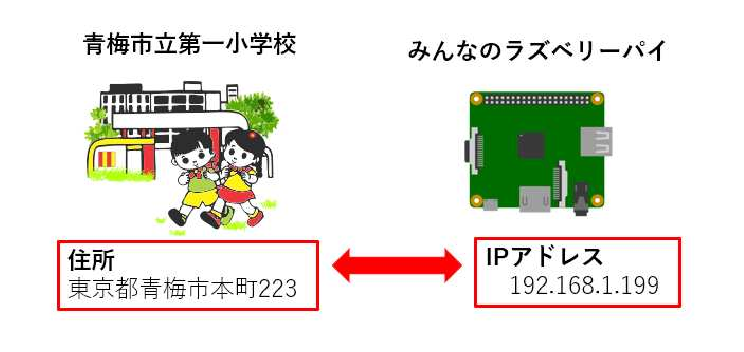
\includegraphics[width=0.8\textwidth]{text07-img/ome7-img003}


\bigskip


\bigskip


\bigskip





\centering
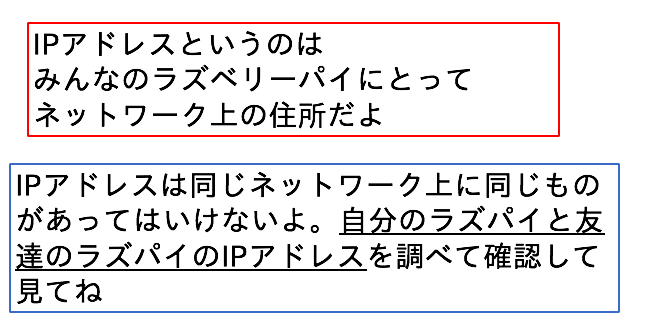
\includegraphics[width=0.8\textwidth]{text07-img/ome7-img004.png}
\flushleft


\bigskip


\bigskip


\bigskip


\bigskip


\bigskip

IPアドレスはラズベリーパイのネットワーク上の住所に当たるものです。一つのネットワークではIPアドレスは同じものがあってはいけません。例えば、配達する人は同じ住所が世界中にあればどこへ配達したらよいかわからなくなってしまいます。インターネットの場合も同じです。なのでIPアドレスは同じではいけません。ですが、例外として他のローカルIPアドレスでは同じになってしまうことはあります。%\textbf{例題7−1で自分のラズベリーパイのIPアドレスを調べましょう}

\clearpage\subsection*{\bfseries 1−3 グローバルIPアドレスとローカルIPアドレス}\label{P:slide_p12}
IPアドレスにはグローバルIPアドレスとローカル(プライベート)IPアドレスという二つに分けられます。



\centering
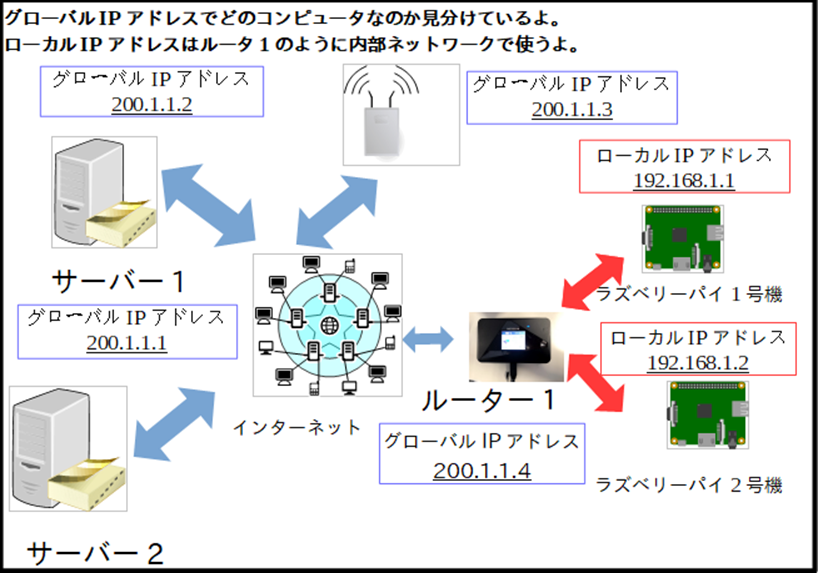
\includegraphics[width=15.0cm]{text07-img/ome7-img005.png}

\centering
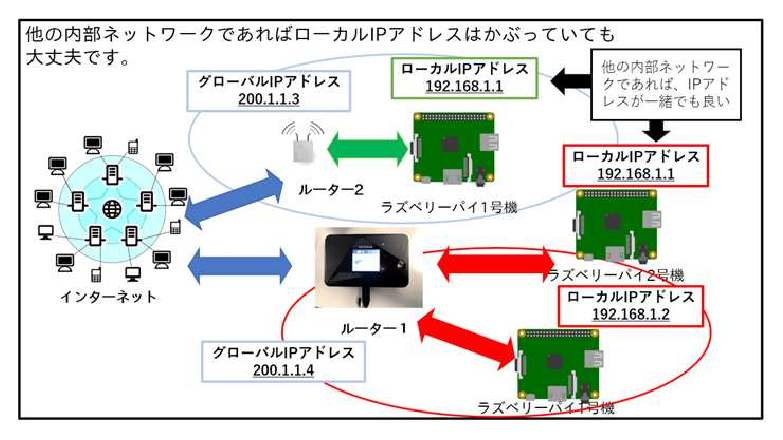
\includegraphics[width=15.0cm]{text07-img/ome7-img006}
\flushleft


{\refstepcounter{Question}\theQuestion ローカルIPアドレスがかぶっても良いときはどのときですか。\label{P:slide_p13} \label{Q:localIP}}\\




{\bfseries
	% \addBlank{答え}
	\vspace*{10mm}
	\underline{答え                            }
}



	\refstepcounter{Exercise}
\clearpage\subsection*{\theExercise IPアドレスを調べてみよう\label{E:checkIP}}

ターミナルにコマンド”hostname
-\texttt{I}”を入力し、自分のラズベリーパイのローカルIPアドレスを確認しよう

{\bfseries
方法}



\centering
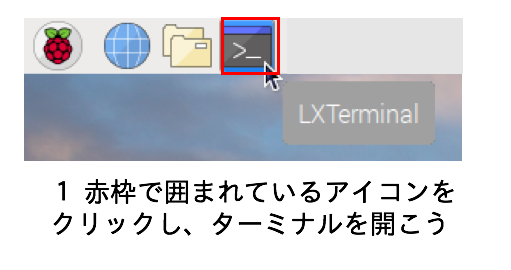
\includegraphics[width=0.85\textwidth]{text07-img/ome7-img007.png}

\centering
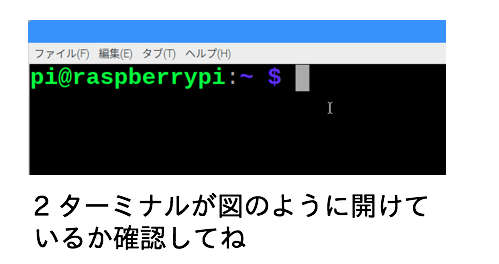
\includegraphics[width=0.85\textwidth]{text07-img/ome7-img008.png}
\flushleft

\clearpage

\centering

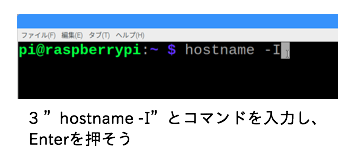
\includegraphics[width=0.85\textwidth]{text07-img/ome7-img010.png}
\centering
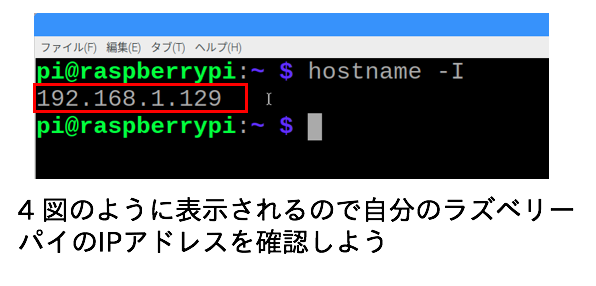
\includegraphics[width=0.85\textwidth]{text07-img/ome7-img009.png}
\flushleft


\bigskip


\bigskip


\bigskip


\bigskip

{\bfseries
	調べた自分のラズベリーパイのIPアドレスを書こう} 

\bigskip


\centering
\begin{tabular}{|p{0.8\textwidth}|} \hline
	\\
	\\
	\\
	\\ \hline
\end{tabular}


\bigskip


\bigskip

\flushleft

{\bfseries
	グループの友達のIPアドレスも教えてもらって書こう}

\bigskip


\centering
\begin{tabular}{|p{0.8\textwidth}|} \hline
	\\
	\\
	\\
	\\ \hline
\end{tabular}


\flushleft


\subsection*{\bfseries }
\clearpage
\textbf{1−4 インターネットのつながりについて知ろう}\label{P:slide_p14}

教室内では無線通信を利用してインターネットを使用しています。第1回目の授業の最初に\ruby{皆}{みな}さんはインターネット\ruby{接続}{せつぞく}をしました。\ruby{実際}{じっさい}にはどこにつながっているかというと下の図のルータです。

\centering
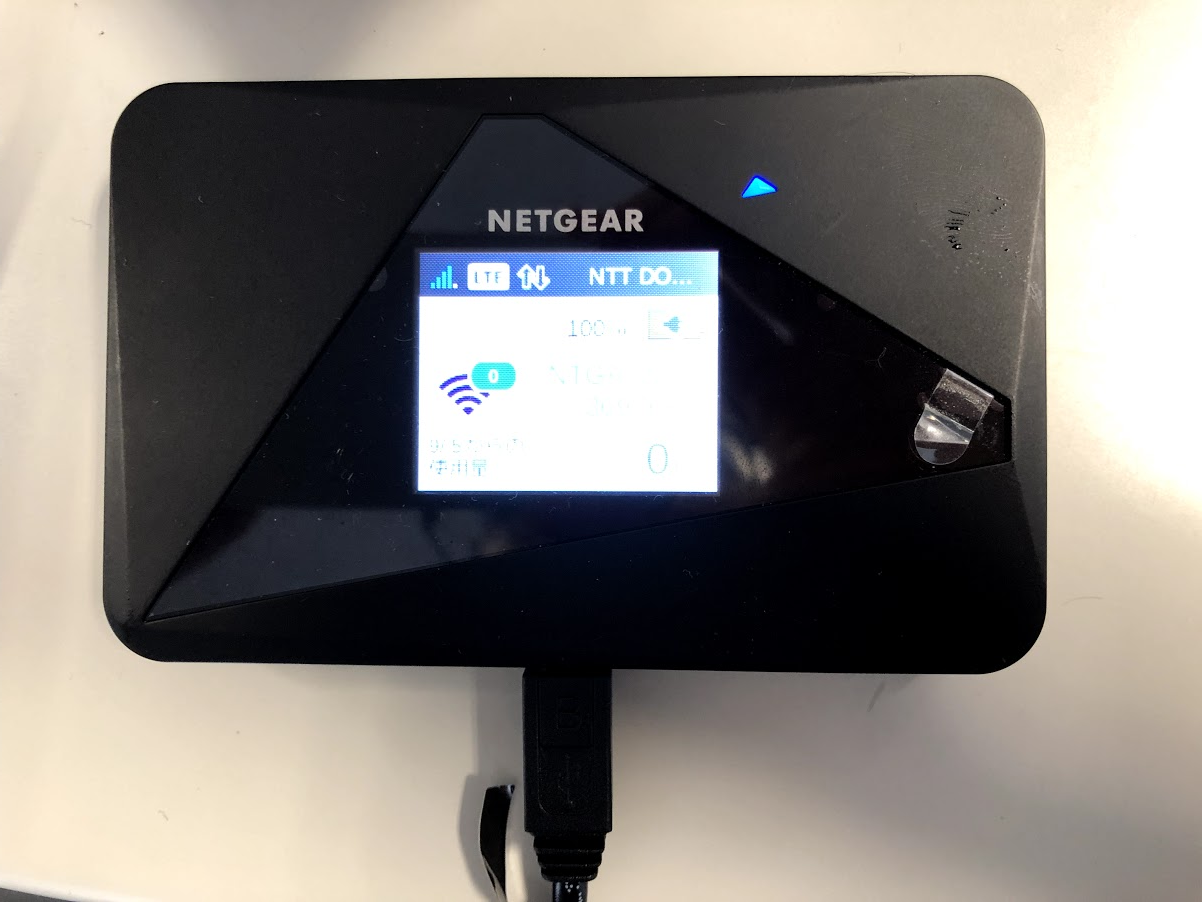
\includegraphics[width=8.186cm]{text07-img/ome7-img011.png}
\flushleft


\bigskip


\bigskip


\bigskip


\bigskip


\bigskip


\bigskip


\bigskip

この機械のおかげで、みんなは教室内でインターネットをすることができているんだ。

どういう原理で、みんなのラズベリーパイでインターネットを使用できているか説明していくよ。

みんなのラズベリーパイは直接インターネットにつながってはいません。一度、ルータを経由しています。このルータのおかげで\ruby{複数}{ふくすう}のラズベリーパイやPCを同時にインターネットにアクセスさせることができるんだ。以下の図がイメージ図だよ。


\bigskip



\centering
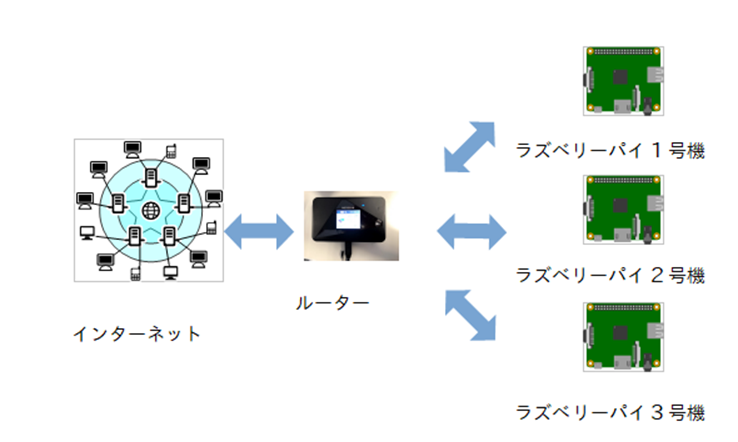
\includegraphics[width=\textwidth]{text07-img/ome7-img012.png}
\flushleft


\bigskip

ではどのようにして複数台のラズベリーパイをインターネットに接続しているのでしょうか。それはルータに\textbf{グローバルIPアドレス}というものを\ruby{割}{わ}り当てて、ルータが他のラズベリーパイの代表として通信を行っています。どういうことかわかりずらいので、図でみていきましょう。



\centering
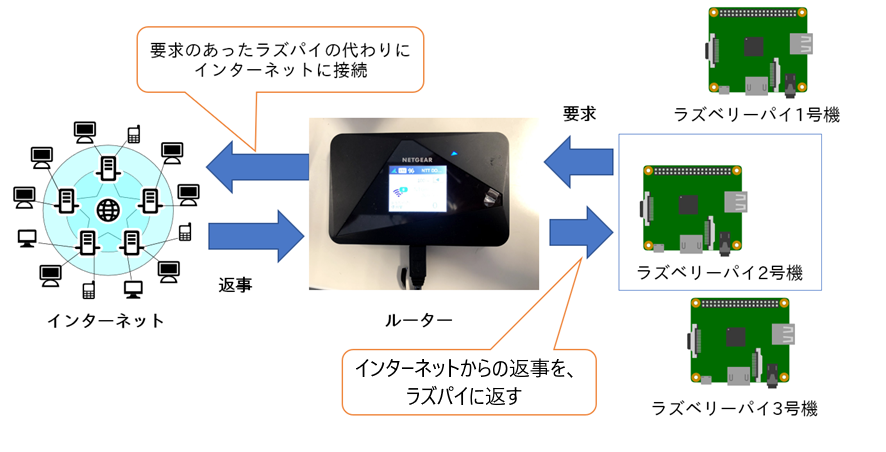
\includegraphics[width=0.9\textwidth]{text07-img/ome7-img013.png}
\flushleft


\bigskip

図ではラズベリーパイ2号機がインターネットにアクセスし、何かしらの webサイトを観たいと要求したとします。その要求はまずルータのところにいき、ラズベリーパイ2号機の代わりにインターネットに接続します。その接続で、ルータはインターネット先から返事をもらい、そのインターネットからの返事をラズパイに返しています。

\centering
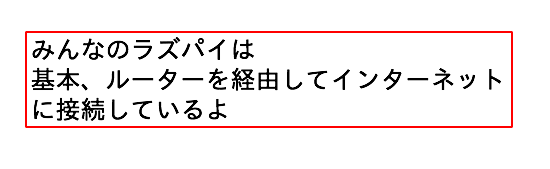
\includegraphics[width=0.9\textwidth]{text07-img/ome7-img014.png}
\flushleft


\bigskip

\clearpage
これだけではうまくいかないことがあります。下の図をみてください。



\centering
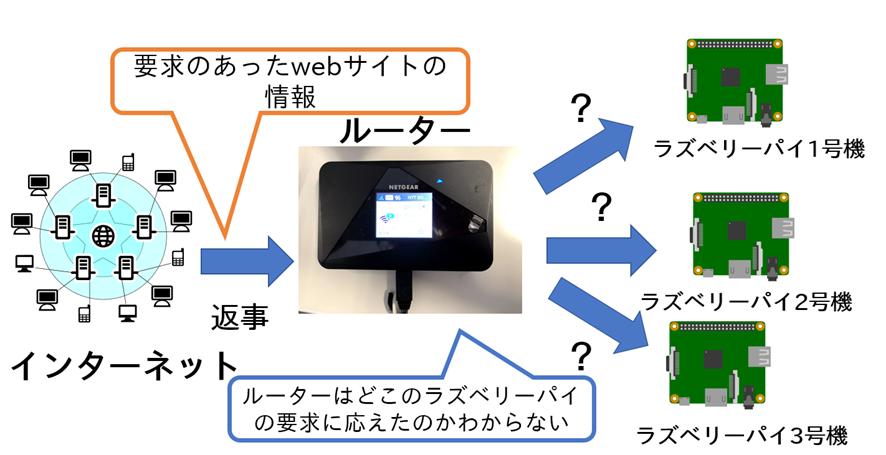
\includegraphics[width=0.9\textwidth]{text07-img/ome7-img015.png}
\flushleft

どれかしらのラズベリーパイからwebサイトへの要求があり、ルータを経由してインターネットに接続します。そのあと、インターネットから要求のあったwebサイトの情報がルータにいきます。ここで問題が発生します。それはいったいのどのラズベリーパイの要求であったのかルータがわからないのです。\ruby{僕}{ぼく}らが、勝手にラズベリーパイ1号機、ラズベリーパイ2号機、ラズベリーパイ3号機と名前をつけて\ruby{判断}{はんだん}していても、そのことはルータはわかりません。そこでIPアドレスというものを使います。

ルータは自分を\ruby{含}{ふく}め、ローカルIPアドレスを割り当てています。このローカルIPアドレスでラズベリーパイを見分けています。


\centering
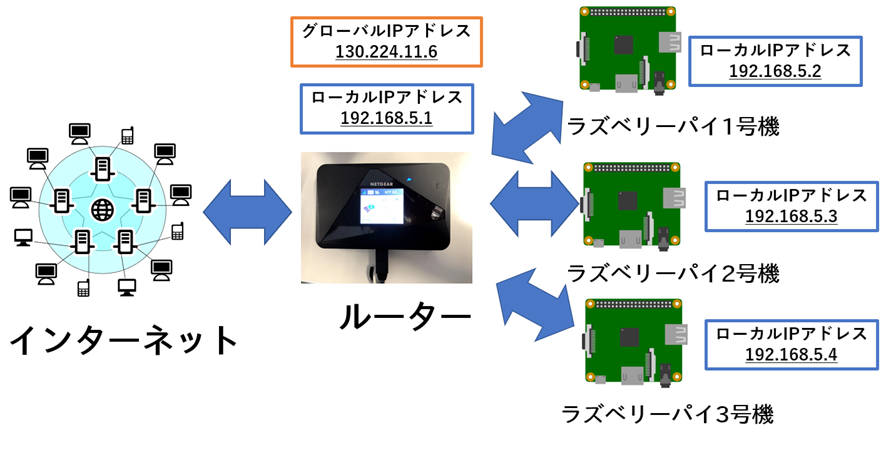
\includegraphics[width=0.9\textwidth]{text07-img/ome7-img016.png}
\flushleft


\refstepcounter{Question}\theQuestion ルータはラズベリーパイたちを見分けるために何を割り当てていますか。\label{P:slide_p15}\label{Q:globalIP}\\

\underline{答え                            }

\refstepcounter{Exercise}


\clearpage\subsection*{\theExercise ポケットWi-FiルータのグローバルIPアドレスを調べよう\label{E:router}}
% \clearpage\subsection*{ポケットWi-FiルータのグローバルIPアドレスを調べよう}
\begin{minipage}[b]{0.58\textwidth}
	ターミナルを開き、”curl	inet-ip.info”とコマンドを入力して、自分のラズベリーパイが接続しているWi-FiルータのグローバルIPアドレスを確認しよう

	curlコマンドはインターネットから情報を取ってくるときに使用します。今回は”inet-ip.info”というサイトからグローバルIPアドレスを調べてターミナルに\ruby{表示}{ひょうじ}させています。webブラウザから”inet-ip.info”にアクセスしてみると右の図のような形でグローバルIPアドレスを確認することもできます。

\end{minipage}
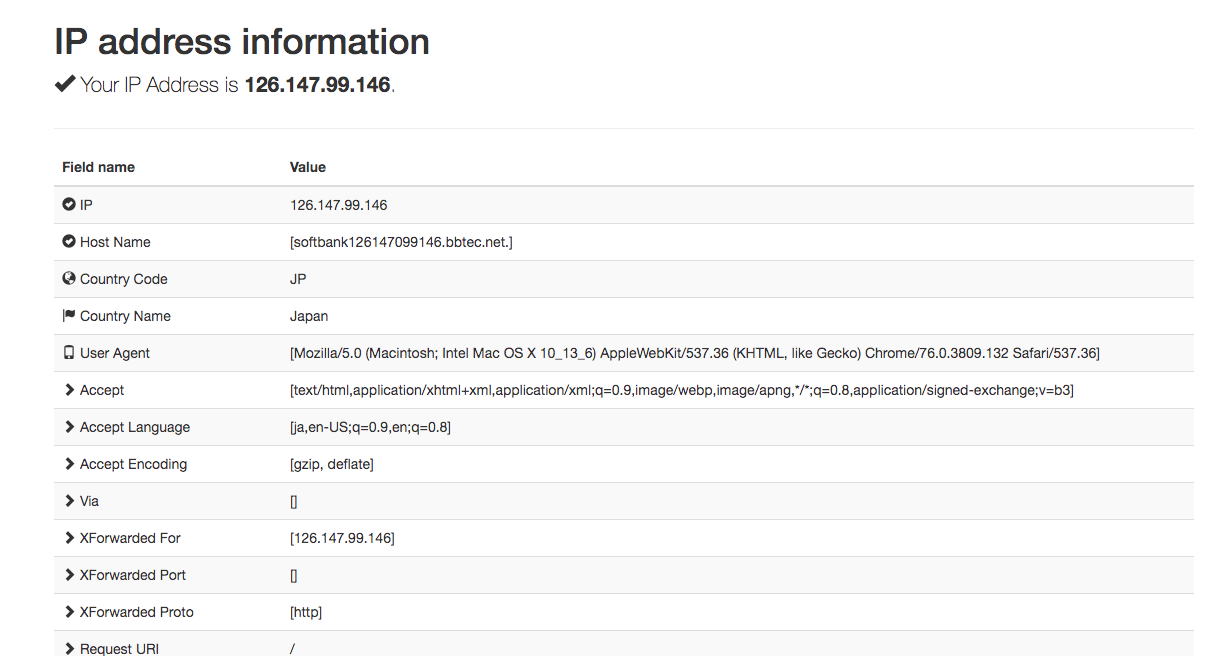
\includegraphics[width=0.4\textwidth]{text07-img/ome7-img017.png}



\bigskip

{\bfseries
	方法}



\centering
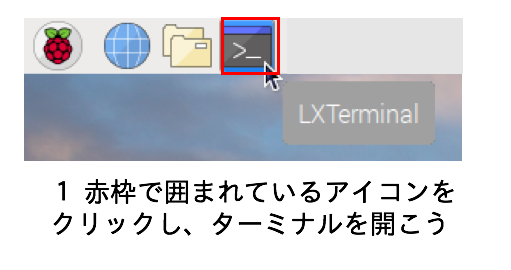
\includegraphics[width=0.85\textwidth]{text07-img/ome7-img007.png}

\centering
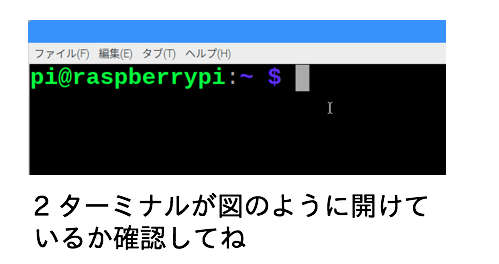
\includegraphics[width=0.85\textwidth]{text07-img/ome7-img008.png}
\flushleft


\bigskip


\bigskip


\bigskip


\bigskip



\centering
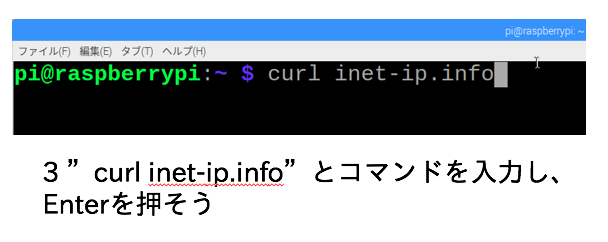
\includegraphics[width=0.85\textwidth]{text07-img/ome7-img018.png}

\centering
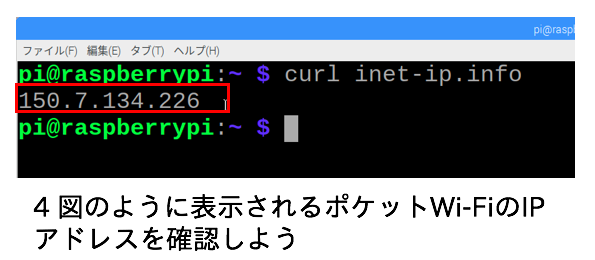
\includegraphics[width=0.85\textwidth]{text07-img/ome7-img019.png}
\flushleft


\bigskip


\bigskip

{\bfseries
	調べたポケットWi-FiのグローバルIPアドレスを書こう}


\bigskip


\begin{table}[htbp]
	\centering
	% \caption{文字タイプ表}
	\begin{tabular}{|c|}
	\hline
	                                                       \\
	                                                       \\
	                                                       \\
	                                                       \\
	                                                       \\

	\hline
	\end{tabular}
\end{table}


\flushleft




\bigskip


\bigskip

{\bfseries
	グループの友達がしらべたポケットWi-FiのグローバルIPアドレスも教えてもらって書こう}



\bigskip


\begin{table}[htbp]
	\centering
	% \caption{文字タイプ表}
	\begin{tabular}{|c|}
	\hline
		                                                       \\
		                                                       \\
		                                                       \\
		                                                       \\
		                                                       \\
	\hline
	\end{tabular}
\end{table}


\flushleft



\bigskip


\bigskip

\clearpage\subsection*{1−5 ポート番号とは}
\refstepcounter{PagePtr}\label{P:port}

\centering
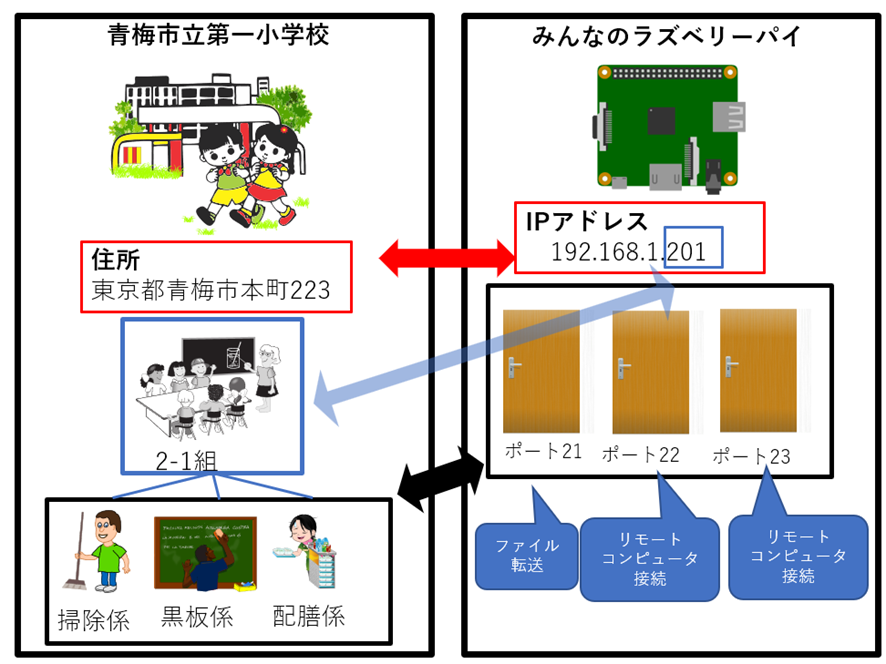
\includegraphics[width=0.85\textwidth]{text07-img/ome7-img020.png}
\flushleft

前のページではみんなはラズベリーパイがどのようにインターネットにつながっているのか理解してくれたと思います。
ここではさらにポート番号について\ruby{知識}{ちしき}を深めましょう。
IPアドレスでは通信相手となる別のネットワークのコンピュータを特定することができます。
しかし、コンピュータでは\ruby{通常}{つうじょう}、多くのプログラム(機能)が動作していて、IPアドレスを指定するだけでは、どのプログラムと接続するかを区別できません。
そこでコンピュータ上の、\underline{どのプログラムと接続するかを指定するためにポート番号が用いられます}。
下の図は小学校を例にしています。

青梅市立第一小学校の住所がみんなのラズベリーパイのIPアドレスに\ruby{対応}{たいおう}しており、IPアドレスの\ruby{末尾}{まつび}の201(青で囲まれている)が小学校のクラスに対応しています。
皆さんの学校でも生徒にはそれぞれ係という役割が\ruby{与}{あた}えられていますね。
例えば、プリントなどの\ruby{配布物}{はいふぶつ}を配る配り係、黒板を使い終わったらきれいにする黒板係、教室の\ruby{窓}{まど}をきれいにする窓ふき係などこれらの係に相当するものがラズベリーパイにもあり、それが\underline{ポート}です。
ポート21はファイル転送用の働きをする\ruby{担当}{たんとう}で、ポート22と23は他のコンピュータに接続する担当です。
ポートには役割がありインターネットの通信はファイル転送であったり、他のコンピュータに接続して\ruby{遠隔}{えんかく}操作したり、webページにアクセスしたりといろいろあります。
なので、その分のポートを用意しておき、役割を与え、対応している役割のときに\ruby{頑張}{がんば}ってもらう仕組みになっています。
みんなのラズベリーパイやパソコン、サーバにはポートは何個あるのか調べてみるのも面白いですね。

\bigskip

\clearpage


\refstepcounter{Question}\theQuestion ポート番号はどのようなことに使われますか。\label{Q:portUsage}\\

\underline{答え                            }

\bigskip

ここでは実際にポートはネットワーク上ではどのように使うのか、下の図を見てみましょう。



\centering
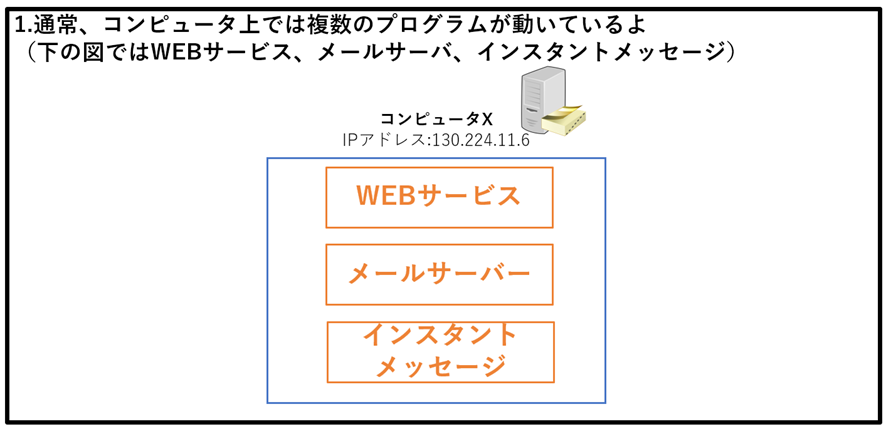
\includegraphics[width=0.97\textwidth]{text07-img/ome7-img021.png}

\centering
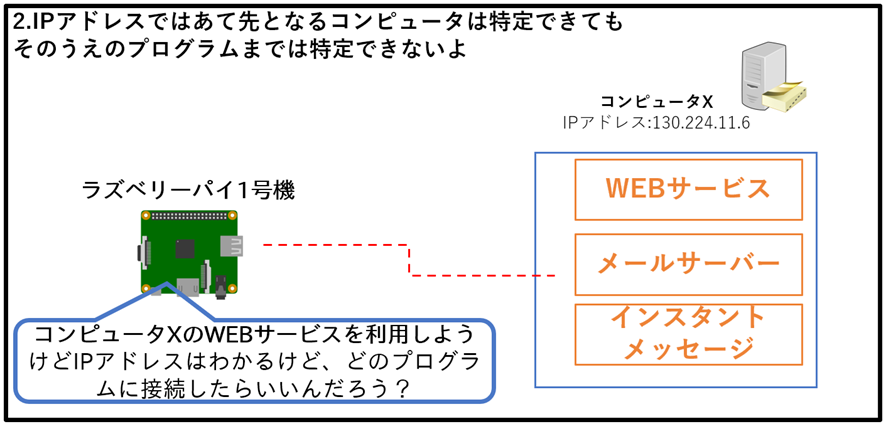
\includegraphics[width=0.97\textwidth]{text07-img/ome7-img022.png}
\flushleft


\bigskip

\clearpage

\centering
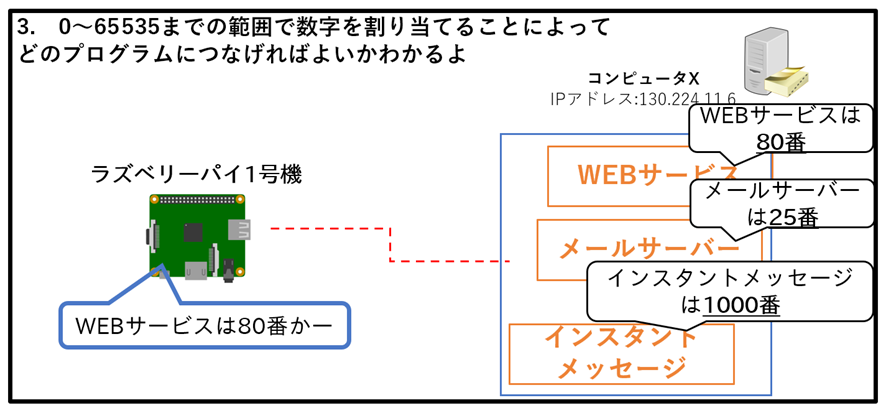
\includegraphics[width=0.97\textwidth]{text07-img/ome7-img023.png}\label{P:slide_p17}



\centering
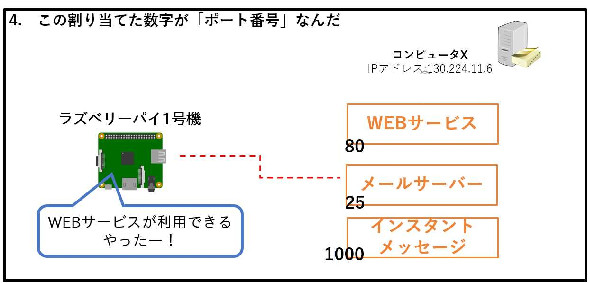
\includegraphics[width=0.97\textwidth]{text07-img/ome7-img024.png}
\flushleft


\bigskip


\bigskip


\bigskip

さらにラズベリーパイ側のポートはラズベリーパイが自動で割当ており、そこからデータを受け取っているよ。


\bigskip


\bigskip


\bigskip



\centering
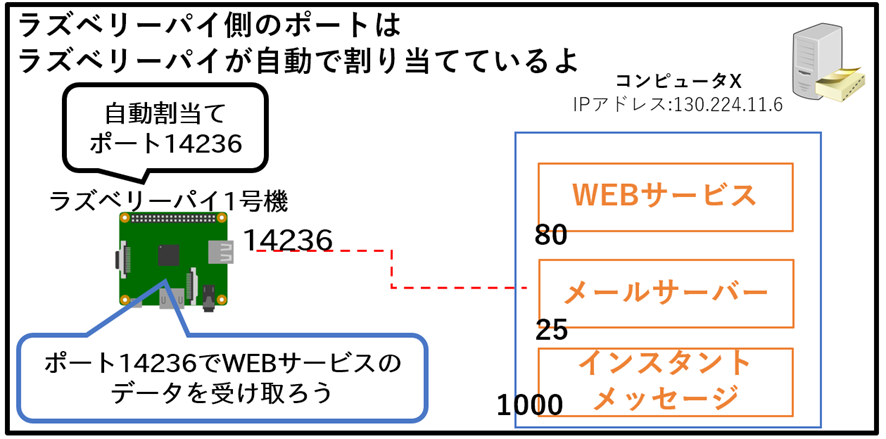
\includegraphics[width=0.97\textwidth]{text07-img/ome7-img025.png}\label{P:slide_p18}
\flushleft

コンピュータXのようにネット上にサービスを\ruby{提供}{ていきょう}するコンピュータを\underline{サーバ}と言います。

ラズベリーパイ1号機のようにサーバからサービスを受けるコンピュータを\underline{クライアント}言います。


\bigskip

これらのポートが今\ruby{現在}{げんざい}どのようなことに使われているのか\textbf{\ref{port}で確認してみましょう。}

\bigskip

{\refstepcounter{Question}\theQuestion コンピュータ上のプログラム(サービス)を判断するためになにが用いられていますか。\label{Q:port}}\\

\bigskip

{\bfseries
	% \addBlank{答え}}
	\underline{答え                            }}

\bigskip
\bigskip
{\bfseries
	ネット上にサービスを提供するコンピュータとネット上のコンピュータからサービスを受けるコンピュータをそれぞれ何といいますか。}

\bigskip
\bigskip
\bigskip


\refstepcounter{Exercise}
\clearpage\subsection*{\theExercise 開いているポートを調べてみよう}
\addtocounter{Exercise}{-1}\refstepcounter{Exercise}\label{port}


ターミナルを開き、”nmap
localhost”とコマンドを入力し、ポートについて知ろう

{\bfseries
方法}



\centering
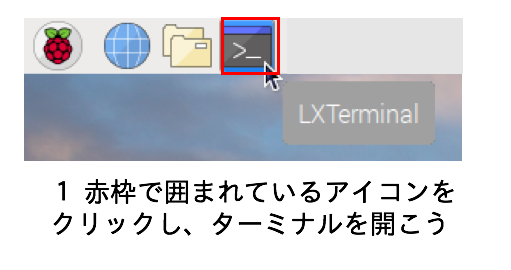
\includegraphics[width=0.85\textwidth]{text07-img/ome7-img007.png}

\centering
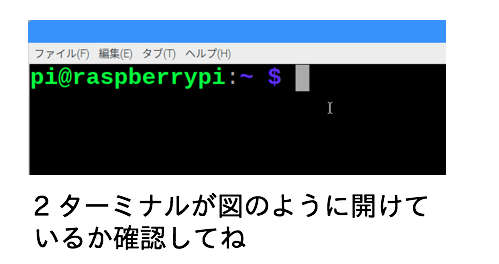
\includegraphics[width=0.85\textwidth]{text07-img/ome7-img008.png}
\flushleft

\clearpage





\centering

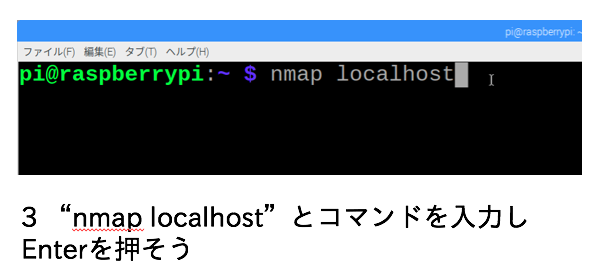
\includegraphics[width=0.85\textwidth]{text07-img/ome7-img032.png}
\bigskip
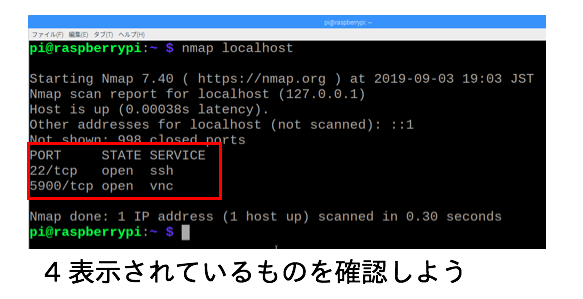
\includegraphics[width=0.85\textwidth]{text07-img/ome7-img031.png}
\flushleft

\bigskip
{\bfseries
	自分のラズベリーパイに表示されたものを下の表に書こう}

\begin{table}[htbp]
	\centering
	% \caption{文字タイプ表}
	\begin{tabular}{|c|c|c|}
	\hline
		PORT           & STATE          & SERVICE          \\
		\hline
		& & \\
		\hline
		& & \\
		\hline
		& & \\
		\hline
		& & \\
		\hline
	\end{tabular}
  \end{table}



{\bfseries
serviceに出てきた言葉をインターネットを使って調べよう。
皆さんにとっては\ruby{難}{むず}しい言葉が多いと思います。
それでも自分で調べてみましょう。
それが知識を深める近道です。\\
ポートが開いていない場合、コマンドは何も表示せず、
改行が起こるだけのこともあります。
}


\clearpage\subsection*{\bfseries コラム DNS(Domain Name System)について}
\refstepcounter{PagePtr}\label{P:DNS}

{\bfseries
	IPアドレスは住所であり、それがわからないとサーバのサービスをうけることはできません。ですが以下の図のようなことが起こることがあります。}

\centering
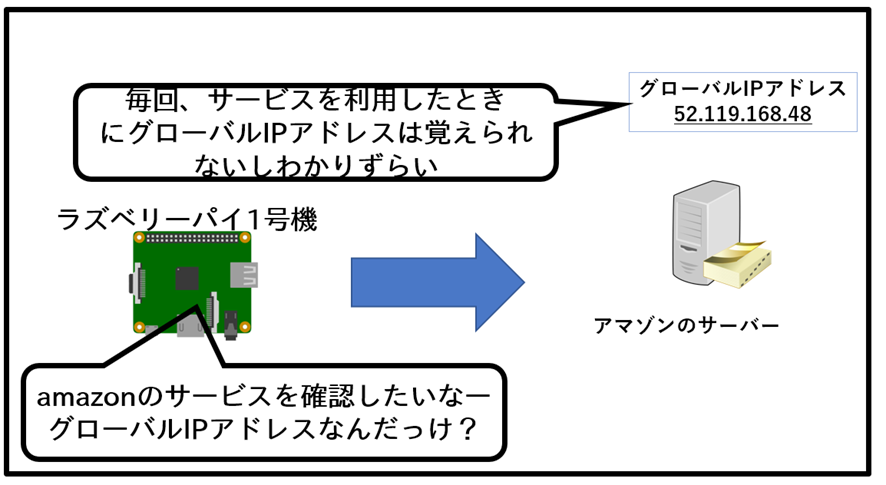
\includegraphics[width=0.97\textwidth]{text07-img/ome7-img026.png}
\flushleft

そこで、DNSサーバと言うものを作り、一度そこに”amazon.co.jp”のグローバルIPアドレスを教えてもらってサーバに接続しています。



\centering
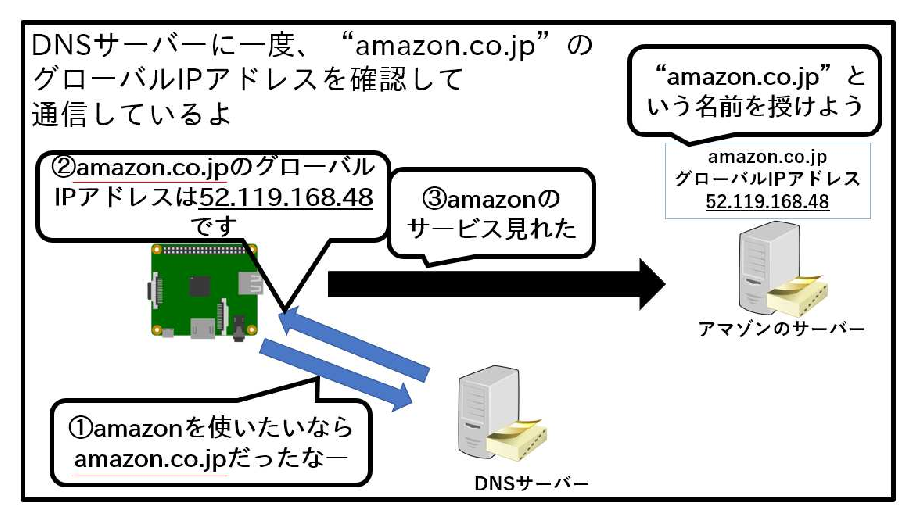
\includegraphics[width=0.97\textwidth]{text07-img/ome7-img027}
\flushleft



\bigskip

\clearpage

\centering
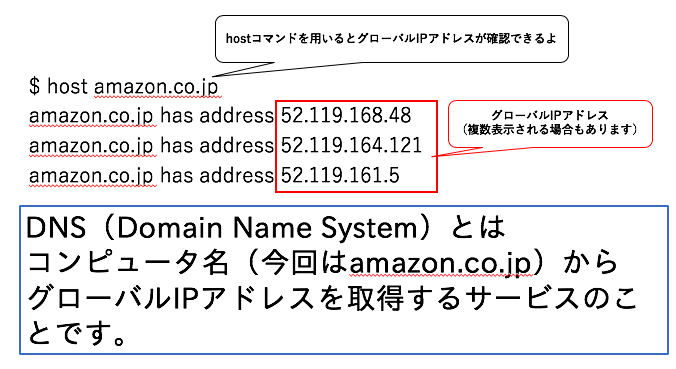
\includegraphics[width=0.8\textwidth]{text07-img/ome7-img028.png}
\flushleft


\bigskip


\bigskip

{\refstepcounter{Question}\theQuestion ターミナルを開き、”dig
	amazon.co.jp”を実行してグローバルIPアドレスを確認しよう。\label{Q:dig}}\\

\bigskip
{\bfseries
	% \addBlank{答え}
	\underline{答え                            }
}
	

\clearpage\subsection*{\bfseries NATについて}

教科書の前のページでローカルIPアドレスとグローバルIPアドレスが存在することを皆さんは知りましたね。ここではもっと細かくIPアドレスを用いたインターネット接続を勉強しましょう。インターネットに接続するコンピュータは自分自身を示すIPアドレスとして世界で\ruby{唯一}{ゆいつ}のグローバルIPアドレスを使わなければならないのです。みなさんのラズベリーパイにはローカルIPアドレスしか割り当てられていませんので、このままではインターネットをすることはできません。そこでNAT(Network
Address
Translation)というものを用います。このNATはルータが行っていて、送信元のローカルIPアドレスをグローバルIPアドレスに変換して通信を行っています。具体的にはどのようになっているのか下の図をみて確認してみよう。



\centering
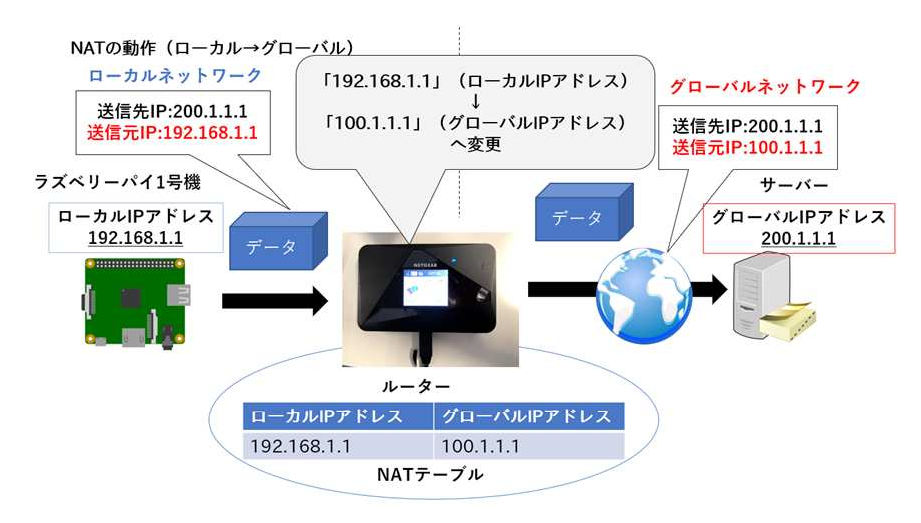
\includegraphics[width=0.9\textwidth]{text07-img/ome7-img029}
\flushleft


\bigskip


\clearpage

ラズベリーパイ1号機からサーバにデータの送信先IPアドレスは200.1.1.1(グローバルIPアドレス)、送信元IPアドレスは192.168.1.1(ローカルIPアドレス)です。NATを行うルータは、プライベートアドレスとグローバルアドレスの\ruby{境界}{きょうかい}に位置しています。ここでルータは、ラズベリーパイから送信されたデータの送信元IPアドレス192.168.1.1を、グローバルIPアドレスの「100.1.1.1」に変換して転送します。このときルータは、その変換情報をNATテーブルに記録しています。この記録が、「返ってくるデータ」、つまりサーバーからラズベリーパイへ送られるデータの転送時に役立ちます。次の図を見てください。



\centering
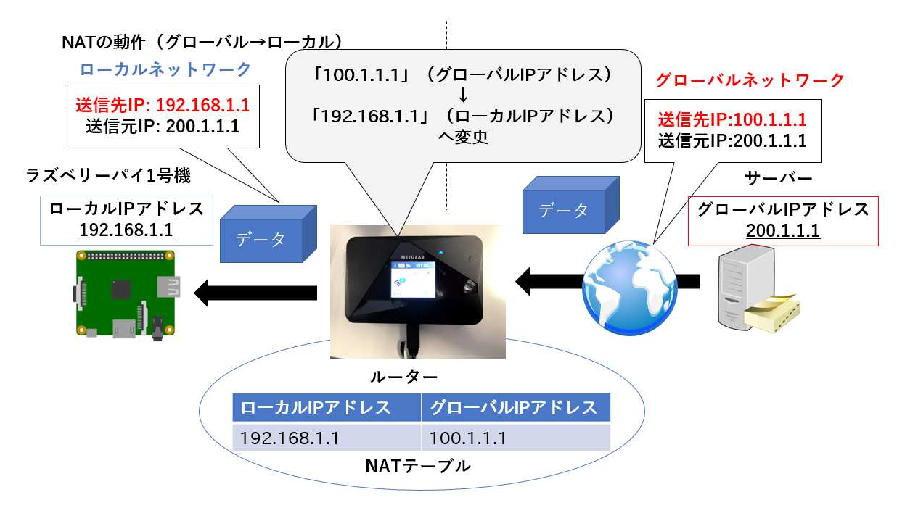
\includegraphics[width=0.9\textwidth]{text07-img/ome7-img030}
\flushleft



\bigskip

サーバーからラズベリーパイへの返事のデータの送信先IPアドレスは「100.1.1.1」、送信元IPアドレス「200.1.1.1」になりますね。データがルータへ転送されてくると、ルータはNATテーブルを確認して、送信元IPアドレスを「100.1.1.1」から元の「192.168.1.1」へ変換します。これにより返りのデータの通信が可能になるのです。NATによって送信元のローカルIPアドレスをグローバルIPアドレスに変換して通信をおこなっているおかげでみんなはインターネットを利用できているんだね。


\bigskip


\bigskip